\section{Problem 3-4}
\label{sec:problem4}

Given $\vect{r}(t_0)$, $\ivect{v}(t_0)$ at $t_0 = 3.93$ min for Case 2, the same Kepler-equation solver is used to find $E$, $\nu$, and $\vect{r}(t)$, $\ivect{v}(t)$ at $t = 1771.58$ min, with $\mu = 398600~\text{km}^3\cdot\text{s}^{-2}$, and the result is compared to \texttt{ode113} at $t_f$ and over a 100-subinterval time series.

\programoutput{outputs/problem4.txt}

\begin{figure}[H]
    \centering
    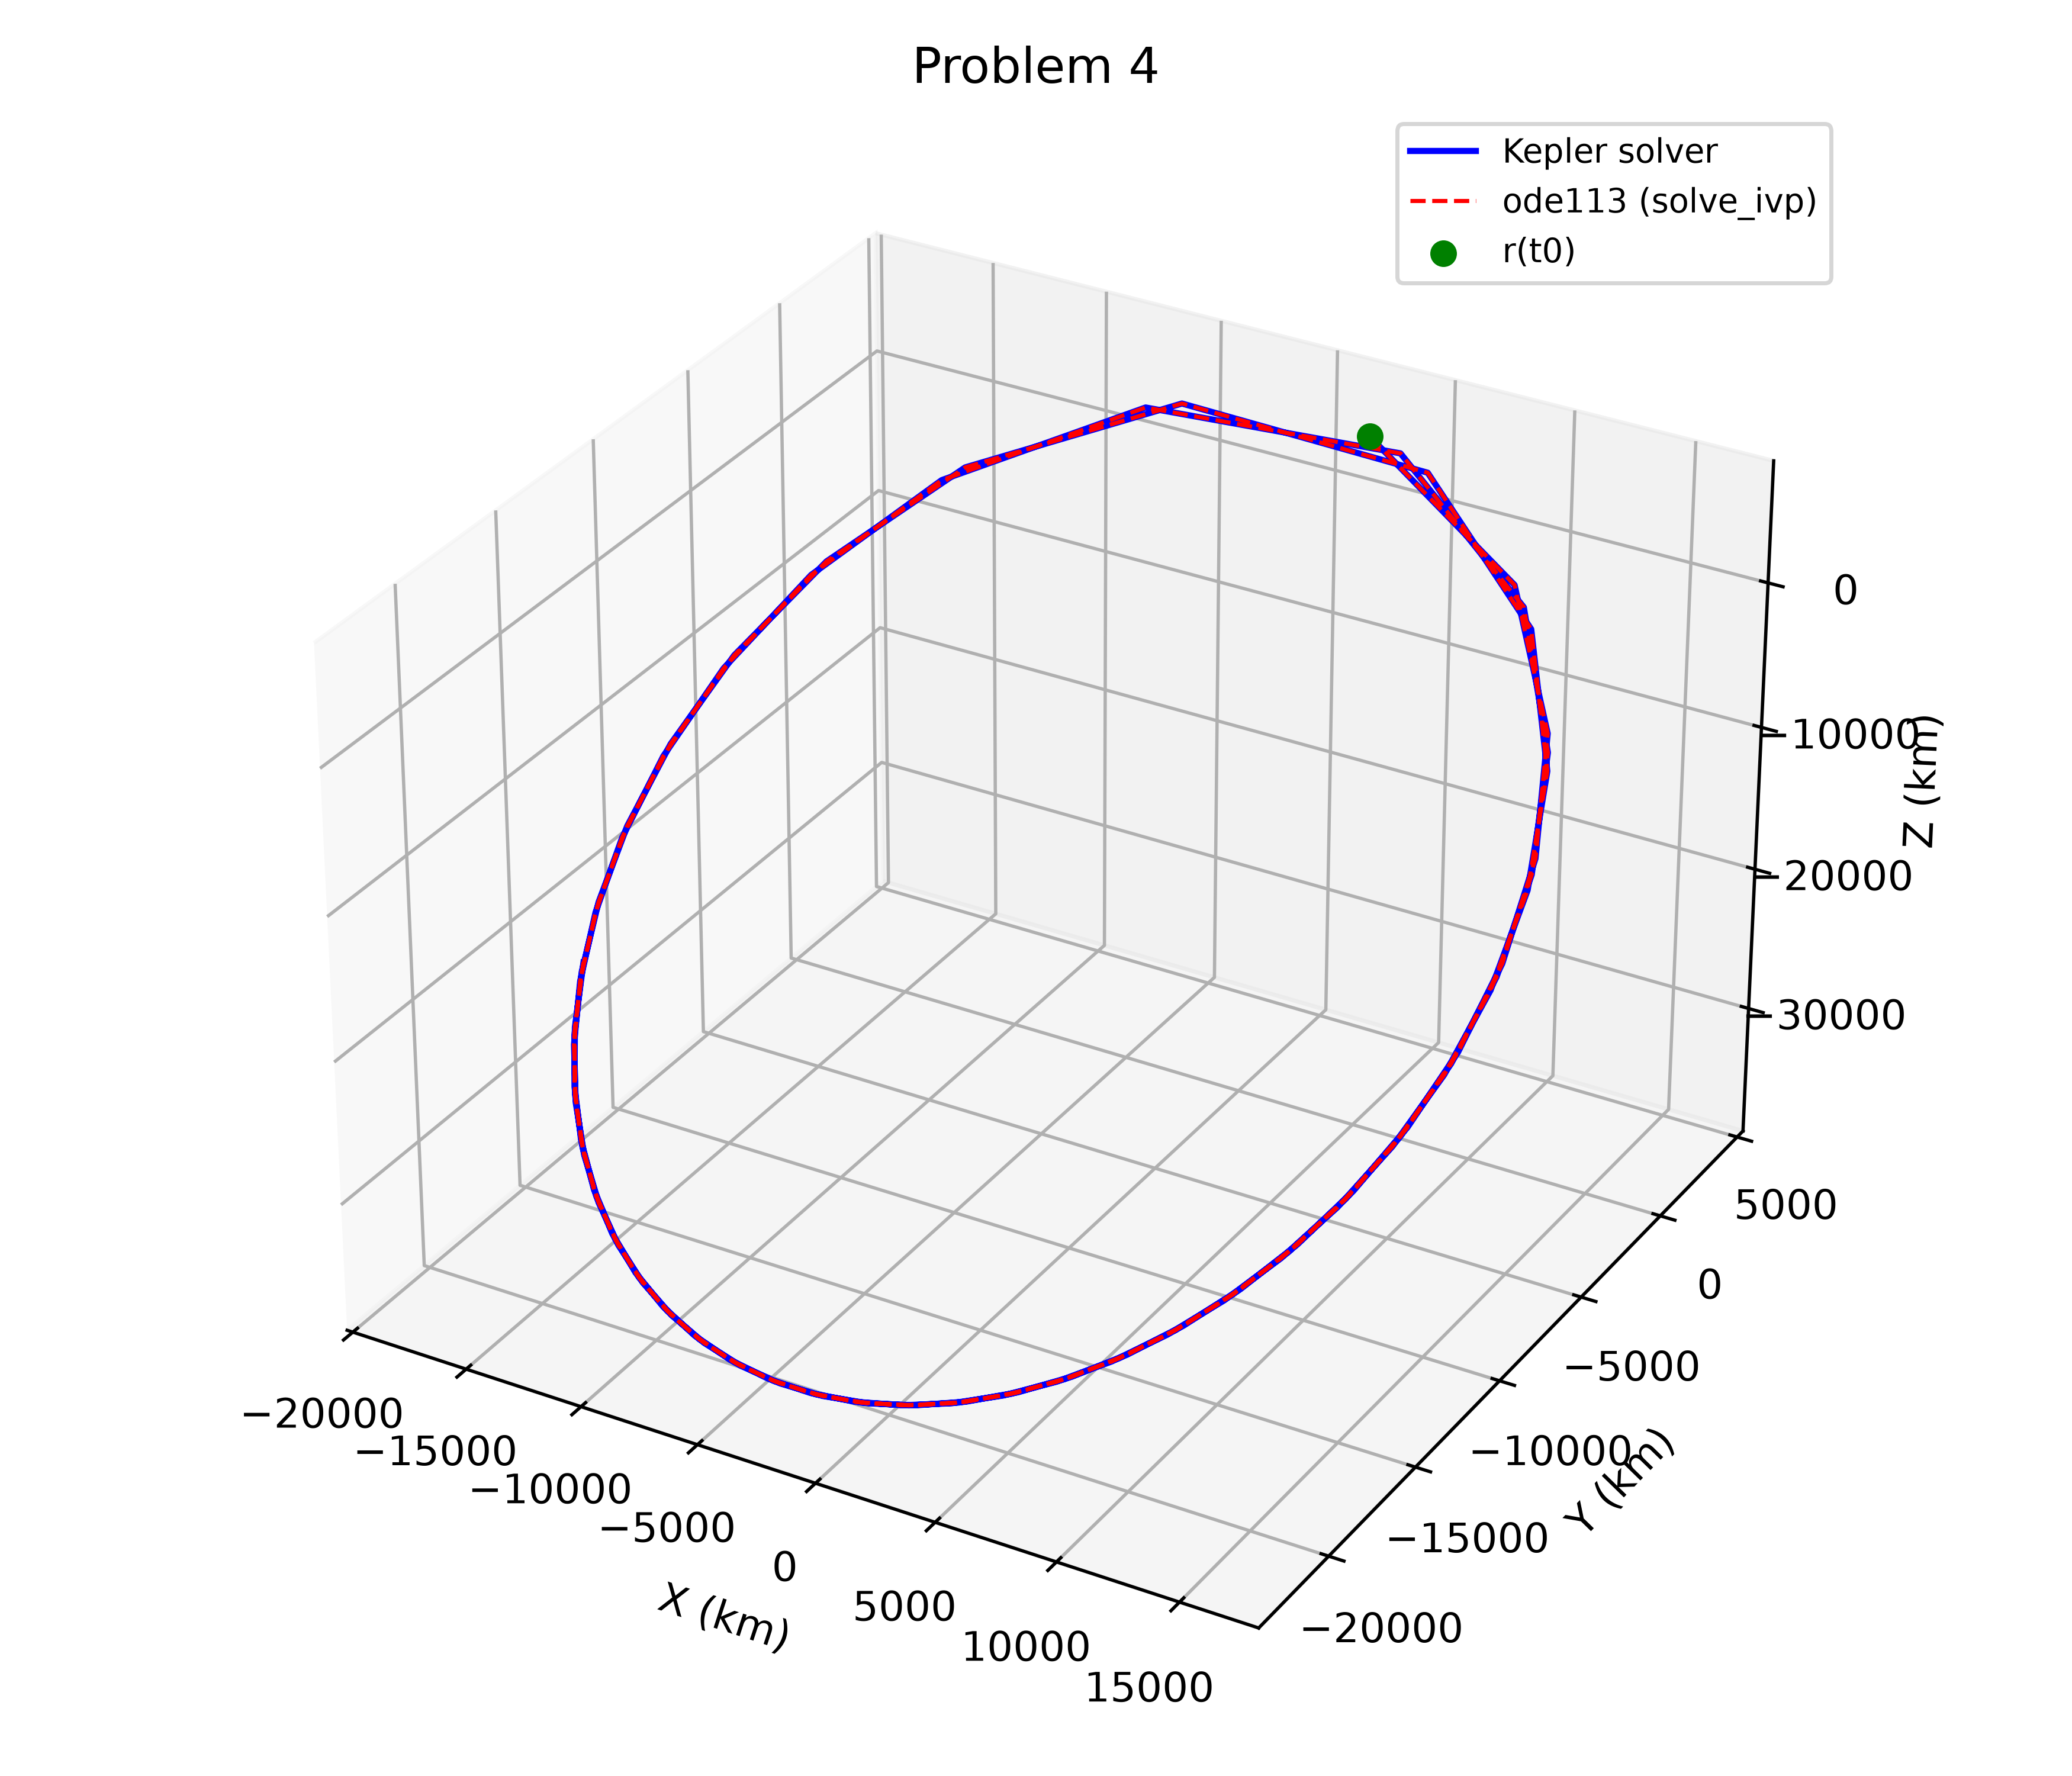
\includegraphics[width=0.75\textwidth]{figures/problem4_orbit.png}
    \caption{PCI position time series from the Kepler solver compared to \texttt{ode113}, Problem 3-4.}
\end{figure}

\FloatBarrier
